\chapter{Long-Context Capability and Decision-Relevant Information}\label{ch:C11}

The 2026 Compaction Cliff study compares compression choices under task-dependent constraints rather than treating retained length as a sufficient quality measure~\cite{zerhoudi2026cliff}. Its conditional results motivate the central distinction developed here: an input can fit a window while losing a decision-critical relation. The mathematical target is preservation of relevant information, with access, reasoning, and computational cost measured separately.

\section{Capacity is a constraint on an inference procedure}\label{sec:C11:capacity}
A context window is an admissible input length, whereas long-context intelligence is a property of a model interacting with a distribution of tasks. The difference becomes operational when an agent must combine an early instruction, a later correction, an external observation, and an unfinished commitment. A successful retrieval of an isolated sentence does not establish that the same model can reconcile those four objects. Conversely, an agent with a modest window may solve a long task by maintaining sufficient state outside that window. Input capacity, effective evidence use, and duration of operation therefore require different measurements.

Let the complete observable history be $H_t=(e_1,\ldots,e_t)$, the query or current decision request be $q_t$, and the model input be $\mathcal C_t=\phi(H_t,q_t)$. The transformation $\phi$ includes serialization, retrieval, truncation, and any instruction or tool-description overhead. A model with token budget $W$ requires $|\mathcal C_t|\leq W$, but this inequality says nothing about whether $\mathcal C_t$ contains the evidence necessary for a correct action. Define a task-dependent evidence set $D_t\subseteq H_t$ and an action loss $\ell(a,Y_t)$. The relevant risk is
\begin{equation}
 R(\phi,\pi)=\mathbb E\!\left[\ell\{\pi(\phi(H_t,q_t)),Y_t\}\right],
 \qquad |\phi(H_t,q_t)|\leq W.
\end{equation}
Here $W$ is the admitted input budget. If the serving interface constrains input and generated tokens jointly, an output reserve must first be subtracted from that joint limit. The distribution in this expectation must identify histories, decisions, environments, and evaluation times. Changing any of them can change the apparent effective context length without changing the architecture.

It is useful to distinguish a capacity failure from an accessibility failure. A capacity failure occurs when a chosen representation cannot fit a sufficient record into the available input. An accessibility failure occurs when a sufficient record is present but the model does not use it correctly. A third category, representation failure, occurs when information was transformed into an ambiguous or incorrect record before the model saw it. These categories imply different interventions: extend the budget, improve the model's use of evidence, or repair the state-construction procedure. Treating them as one phenomenon encourages expensive remedies that miss the responsible subsystem.

The transformer construction makes every permitted earlier token potentially available through attention, but potential connectivity is not reliable semantic access~\cite{vaswani2017attention}. Position encodings, training distributions, intermediate representations, decoding, and instructions all mediate that access. A systems description should therefore specify the input length, the position of decisive evidence, the number of distracting or contradictory records, and the logical operations required to derive the action. The phrase ``supports a long context'' becomes scientifically informative only after those conditions are fixed.


\section{A sufficiency criterion for retained state}\label{sec:C11:sufficiency}
The strongest justification for discarding history is that the retained representation preserves all information needed for the decisions being evaluated. Suppose $Y$ is a finite-valued target and $Z=\phi(H)$ is a deterministic state representation. Under logarithmic loss, the optimal expected losses using $Z$ and $H$ are $H(Y\mid Z)$ and $H(Y\mid H)$, respectively. Their difference is
\begin{equation}
 H(Y\mid Z)-H(Y\mid H)=I(Y;H\mid Z)\geq0.
 \label{eq:C11:informationloss}
\end{equation}
This is an information-theoretic deduction, not an empirical result about an existing agent. It assumes optimal conditional predictors and a fixed target distribution. Equality means that $Z$ is sufficient for predicting $Y$ relative to $H$. A fluent summary can have high semantic similarity to the original text while leaving this conditional mutual information strictly positive.

For sequential control, preserving the current answer is weaker than preserving future decisions. Let $X_t$ be the environment state and let $Z_t$ summarize observable history. A sufficient control state should support the conditional distribution of future observations and rewards under relevant action sequences. One possible exact condition is
\begin{equation}
 P(O_{t+1},R_t\mid H_t,a)=P(O_{t+1},R_t\mid Z_t,a)
\end{equation}
for every action under consideration, together with a recursively valid update of $Z_t$. This condition is demanding because the environment is partially observed and the action set may change when new tools become available. A task-oriented summary is usually an approximation to this condition rather than a demonstrated sufficient statistic.

Consider a repository task whose earlier history contains a requirement to preserve an undocumented compatibility behavior. A summary that retains the current implementation plan but omits that requirement may support the next edit and still fail a later regression check. The target variable in Eq.~\eqref{eq:C11:informationloss} must then include that later check. If evaluation asks only for the next action, the compression can appear lossless even though it removes information necessary for task completion. Horizon and target definition are part of any claim about retained information.

An approximate decision bound can be stated without assuming optimal language modeling. Suppose two histories represented by the same $z$ induce future-trajectory laws differing by at most $\epsilon\in[0,1]$ in total variation under every evaluated policy. For the same return functional $G$ taking values in $[-V_{\max},V_{\max}]$, their expected returns differ by at most $2V_{\max}\epsilon$. If instead $G\in[0,V_{\max}]$, the bound is $V_{\max}\epsilon$. These follow from the range of a bounded function and the definition of total variation. The observation motivates evaluating behaviorally distinct histories that collapse to the same summary. It does not provide a practical certificate unless the required uniform bound can be estimated or established from environment structure.

The engineering consequence is to make discarded distinctions explicit. Preserve obligations, authorization, unresolved alternatives, evidence provenance, and invalidated assumptions as typed state rather than relying on a generic narrative summary. Exact sufficiency may be unattainable, but the system can identify which future decisions its representation is intended to support and which distinctions it knowingly loses.

Information availability and a fixed model's competence must be separated when interpreting a full-history baseline. For a finite action space and bounded loss, define the Bayes risk under information $Z$ by
\begin{equation}
 R^*(Z)=\mathbb E\!\left[\min_a\mathbb E[\ell(a,Y)\mid Z]\right].
\end{equation}
If $Z=\phi(H)$, a policy with access to $H$ can imitate every $Z$-measurable decision rule, so $R^*(H)\leq R^*(Z)$. An observed improvement after deleting context therefore concerns the evaluated model, assembly procedure, and resource constraint; it does not show that removing information improves the unrestricted optimal decision. Compression can reduce distraction or make a finite computation feasible while still discarding information that another policy could use. This distinction is essential when attributing gains to a 2026 editor rather than to a weaker full-history implementation.



Figure~\ref{fig:C11:information-policy-risk} isolates the mechanism and its stated information boundaries.
\begin{figure}[!htbp]
\centering
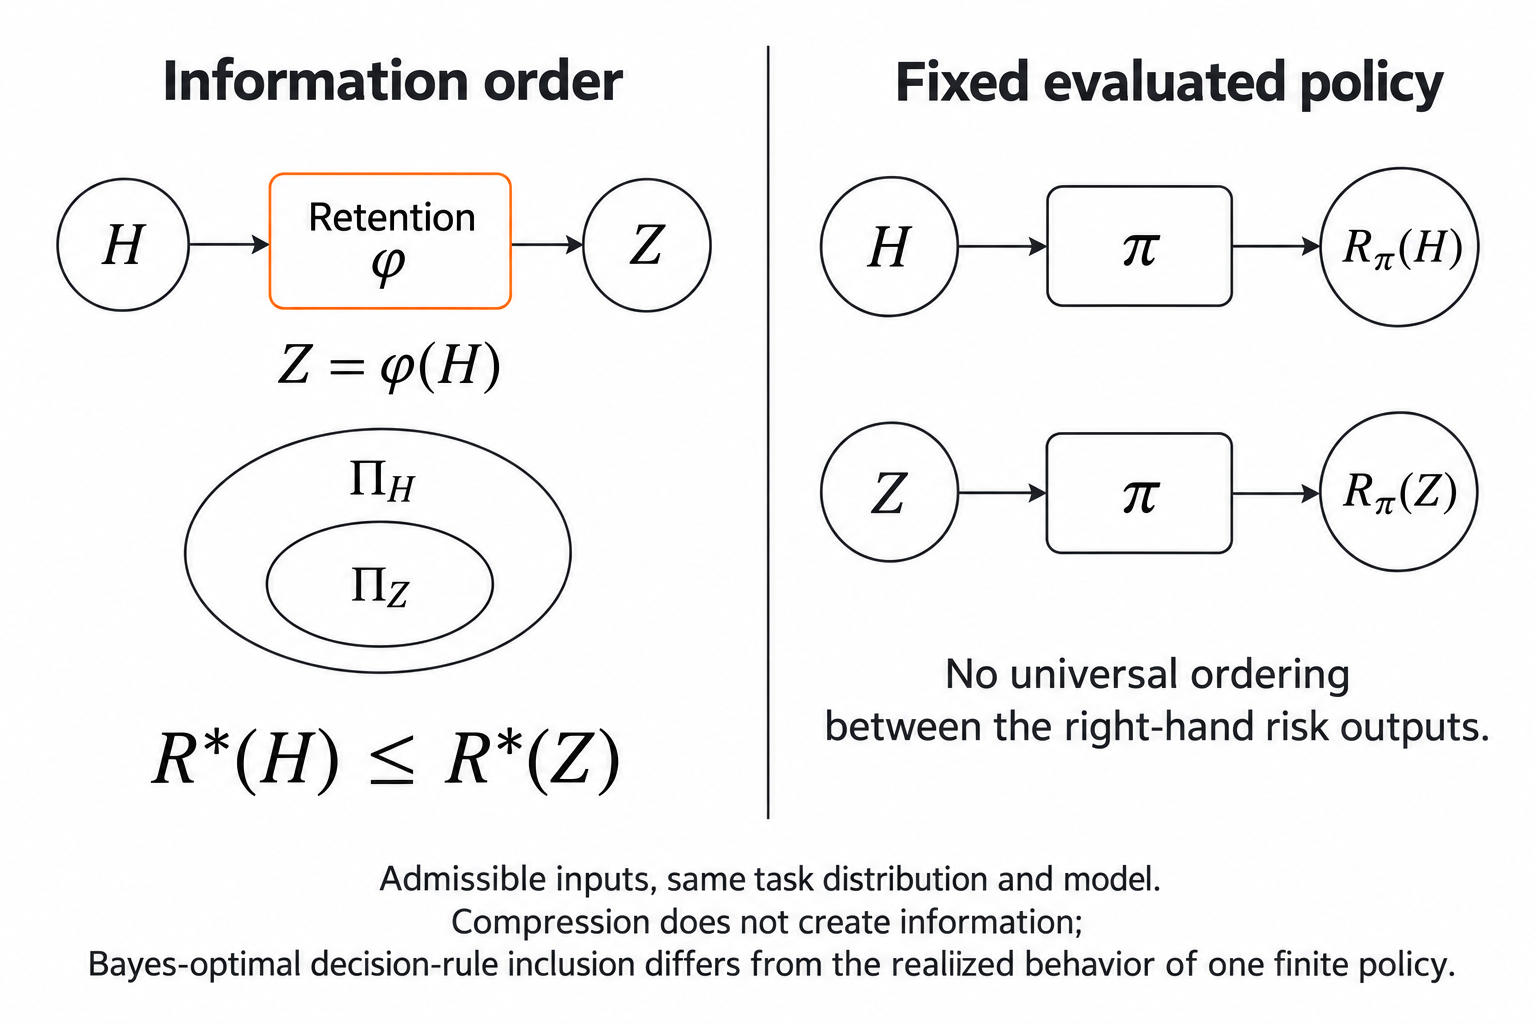
\includegraphics[width=\linewidth]{book/figures/assets/F11review.png}
\caption{Deterministic retention restricts the available decision rules, so $R^*(H)\leq R^*(Z)$ under the stated Bayes-risk assumptions. A fixed model can nevertheless perform better on a compressed view because computation, distraction and serialization affect its realized behavior. The right-hand risks have no universal ordering. This original schematic contains no empirical comparison.}
\label{fig:C11:information-policy-risk}
\end{figure}

\section{Position effects and compositional difficulty}\label{sec:C11:geometry}
Length is only one coordinate of task difficulty. A useful workload specification includes evidence distance, evidence density, distractor similarity, the number of required joins, contradiction depth, and the delay between observation and consequence. Evidence density is the fraction of input that contributes to a correct answer. Low density stresses selection; high density with many dependencies stresses integration. Two inputs of equal token length can therefore create different computational demands.

Lost in the Middle provides evidence that information placement can affect model performance in its tested retrieval and question-answering settings~\cite{liu2023lostmiddle}. RULER and LongBench broaden long-context evaluation through controlled and heterogeneous tasks~\cite{hsieh2024ruler,bai2023longbench}. Their central methodological value here is to make context use observable under specified tasks. They do not establish a universal conversion from advertised token capacity to a reliable operating horizon. Synthetic retrieval, document question answering, and multi-step interactive execution expose overlapping but different failure modes.

The pinned RULER implementation makes several controls inspectable. In \path{scripts/data/synthetic/niah.py}, \path{generate_input_output} varies needle keys, values, queries, distractors, and insertion positions; \path{generate_samples} uses the selected tokenizer and reserves generated tokens and model-template overhead while fitting inputs. The standalone \path{scripts/pred/call_api.py} prediction path appends the stored answer prefix before dispatch. In \path{scripts/eval/evaluate.py}, \path{run_evaluation_per_task} applies the task metric and separately counts empty predictions~\cite{cumulative_a_ruler_repo_20261029}. Preserve the exact rendered input, tokenizer, seed, target position, and generation reserve when comparing lengths. The inspected prediction helper retries exceptions without a finite retry limit, and the evaluator skips absent task files after printing a warning. A reproducible adaptation should impose a declared deadline, reconcile expected and completed task identifiers, and retain failed requests in its accounting. These are implementation obligations; this static benchmark does not itself certify session continuity or correct external effects.

To separate these effects, construct a family of tasks with fixed decisive records and systematically permute their positions while keeping total length constant. Next, increase distractor similarity without changing the decisive records. Finally, change the number of relations needed to connect the records. The resulting response surface $s(L,d,k,\rho)$ records success as a function of length $L$, evidence distance $d$, join count $k$, and distractor parameter $\rho$. A length-only curve is a projection of this surface and can conceal strong interaction effects.

Repeated facts require special care. Repeating a constraint near the decision can improve accessibility while changing the workload's redundancy. If a long-context method benefits from explicit reminders, that result should be distinguished from recovery of a unique distant fact. Likewise, a task that includes both a stale fact and a corrected fact tests temporal interpretation as well as retrieval. An answerer can retrieve both perfectly and still resolve their authority incorrectly. Position permutations must preserve timestamps and source roles or the experimental manipulation changes the intended semantics.

Compositional difficulty also interacts with output format. Choosing a cited answer from a small candidate set can be easier than synthesizing an executable action with multiple arguments. An agent must often retrieve an entity, infer its current state, select a tool, satisfy a schema, and respect an authorization boundary. Evaluation that terminates after entity retrieval measures only the first component. For expert comparison, the action-generation stage should be retained, and failures should be attributed to evidence access, reasoning, argument construction, or execution.

An informative negative control inserts irrelevant but lexically attractive records whose instructions conflict with the user task. The model should recognize these as data rather than authority. This extends context evaluation toward the security analysis in Chapter~\ref{ch:C28}. Success under benign distractors does not imply robustness when retrieved content attempts to redefine the task or rewrite the memory policy.


\section{Training distributions and length generalization}\label{sec:C11:training}
Length generalization depends on more than the numerical range of a position encoding. Training establishes distributions over token positions, document boundaries, dependency lengths, and tasks. Increasing an inference limit changes the region in which those learned mechanisms operate. Rotary or recurrent positional constructions address parts of this problem, but an architectural ability to represent a position does not by itself demonstrate competent reasoning at that position~\cite{su2021roformer,dai2019transformerxl}.

For an agent, training must additionally expose the model to histories with interrupted plans, corrected observations, failed tool calls, and records that have become irrelevant. A long concatenation of independent documents is not equivalent to a coherent interaction trajectory. The latter contains dependencies between what the policy observed, what it attempted, what the environment changed, and what remains unresolved. Training data that omit these distinctions can reward answer extraction while failing to teach durable task-state maintenance.

Let $p_{\mathrm{train}}(L,K,T)$ describe training examples by length, dependency complexity, and interaction type, and let $p_{\mathrm{deploy}}$ describe deployment. Reporting only a maximum training length suppresses shifts in the other coordinates. A model may encounter deployment histories within the trained length range but outside the trained distribution of corrections or tool-output redundancy. The appropriate claim is then distribution-specific performance, not unrestricted length generalization.

A defensible extension experiment holds architecture and total training compute fixed where feasible, varies the long-sequence curriculum, and evaluates both short and long tasks. The short-task control detects capability tradeoffs, while the long-task suite distinguishes retrieval from integration and interactive continuity. If extra long-sequence training also increases the token budget or improves data quality, the comparison must identify those additional factors. A recovery phase after agentic post-training has a real compute cost and should not disappear from the accounting boundary.

Contamination controls operate at the level of both documents and tasks. Removing exact benchmark documents does not rule out exposure to paraphrased questions, released solutions, or public environment traces. For interactive tasks, the environment schema and common solution trajectory can leak even when the surface instruction is novel. Separate held-out entities, templates, environment states, and required action compositions. Record which dimensions were held out and avoid claiming general transfer from a single split.

Implementation should preserve document and event boundaries through packing. If truncation removes the role or timestamp of a message, the remaining content can acquire a different interpretation. Tokenization and serialization are therefore part of the learning distribution. Chapter~\ref{ch:C17} analyzes the stronger problem arising when training reconstructs a different context from the one used during rollout. Long sequences can be correctly packed in memory and still be conditionally wrong for learning.


\section{Computation and memory over an interaction horizon}\label{sec:C11:resources}
Assume a decoder with $n_\ell$ layers, hidden width $d$, $h_{kv}$ key-value heads, equal key and value head dimension $d_h$, and $b$ bytes per cached scalar. Assume the same cache shape at every layer and full residency of every visible token; latent caches and layer-specific or sliding-window caches require their own accounting. Ignoring allocator overhead, the cache for one sequence of $L$ tokens occupies
\begin{equation}
 M_{KV}=2n_\ell Lh_{kv}d_h b.
 \label{eq:C11:kv}
\end{equation}
The factor two accounts for keys and values. This expression excludes model weights, activations, page metadata, workspace, and fragmentation. Grouped-query attention changes $h_{kv}$; changing the total query-head count without specifying key-value sharing is insufficient for memory accounting~\cite{ainslie2023gqa}. Cache paging changes allocation behavior rather than the semantic amount of remembered evidence~\cite{kwon2023pagedattention}.

For dense attention, an incremental decode step reads a growing cache and performs attention against the visible prefix. A simplified traffic model is $B_t\simeq\kappa M_{KV}(L_t)$, with $\kappa$ representing actual cache access, reuse, and implementation overhead. The bandwidth lower bound $B_t/\beta$ assumes an effective bandwidth $\beta$ and cannot predict observed latency without accounting for compute, synchronization, batching, and competing traffic. Peak device bandwidth is not sustained application bandwidth.

The interaction horizon introduces cumulative costs. If each tool turn contributes $u$ input tokens and the system repeatedly reconstructs the full history, the total input volume over $T$ turns scales as
\begin{equation}
 \sum_{t=1}^{T}ut=uT(T+1)/2.
\end{equation}
This is an analytic count under equal-sized turns and no reusable prefix accounting. Prefix caching can reduce repeated computation, while billing rules may count tokens differently. The expression therefore diagnoses a growth pattern rather than an invoice. A bounded working context of size $W$ changes the repeated-input term toward $O(TW)$ but introduces storage, retrieval, editing, and error-recovery costs.

Long-context serving also creates capacity competition. A scheduler holding a large inactive session can reduce concurrency for short requests. Evicting that session's cache saves device memory but may incur a costly prefill when it resumes. The correct objective depends on the workload mixture and service-level constraints: minimize mean cost, maximize throughput, or control tail latency. A policy optimized for average token throughput can be undesirable when a few latency-sensitive tool decisions gate an entire workflow.

Latency should be decomposed into queueing, context construction, prefill, generation, tool execution, and validation. These components are not independent. Large contexts can increase queueing through resource contention; additional retrieval can reduce prefill but add a network round trip; compression can reduce the next call yet increase retries after information loss. Report distributions over complete tasks and retain timeouts. Measuring only successful completions introduces survivorship bias into both latency and cost estimates.

The practical design question is consequently when additional retained context produces enough decision value to justify its full systems cost. That tradeoff depends on the probability that distant evidence becomes decisive, the cost of reacquiring it, and the consequences of forgetting it. Uniform retention and uniform eviction are both coarse approximations to this decision problem.


\section{Experimental designs that isolate context use}\label{sec:C11:experiments}
A proposed long-context evaluation should begin with matched information access. Full-history, retrieval, and summary systems should receive the same underlying evidence, tools, model version, and authorization. The comparison then varies only how evidence reaches the model. A second experiment can permit learned context control, but its training and search costs should be reported separately. Otherwise, architectural selection effects become entangled with an additional optimization budget.

Recent work makes these distinctions concrete. The Compaction Cliff classifies knowledge by type and applies separate operators for compaction, decomposition, and retrieval, retaining recognized constraints under type-specific rules~\cite{zerhoudi2026cliff}. Its guarantees depend on constraint classification, applicable scope, feasible budgets, and verification; they are not unconditional preservation of every real safety requirement. Its behavioral retail comparison is not token-matched, and some reference labels are model-generated. Those qualifications prevent an observed advantage from being assigned solely to typing. The preprint was available before the cutoff even though its listed conference dates fall later.

The methodological conflict is useful. Uniform summarization assumes that one semantic compression objective is adequate across records, whereas typed retention treats some distinctions as constraints that should survive with stronger fidelity. The latter can preserve a rare prohibition even when a relevance score prefers repeated descriptive content. It can also fail if the classifier mistakes a declarative fact for ordinary background or assigns an inappropriate scope. A test of constraint preservation should therefore vary grammatical form and authority independently of content frequency.

Two 2026 surveys supply organizing lenses rather than independent experimental confirmation. The rate--distortion view groups several forms of context-derived compression under budget and downstream-utility tradeoffs~\cite{colaco2026ratedistortion}. The October selective-memory survey distinguishes information participating in computation from stored information that can later be activated~\cite{gou2026selective}. These taxonomies help align accounting boundaries, but they do not prove that cache eviction, semantic forgetting, and text summarization have identical guarantees. Their state transitions and recovery mechanisms remain different.

An original deduction follows from combining these distinctions with the sufficiency criterion: fidelity should be allocated according to the loss of the distinction being removed, while activation cost should be charged when stored evidence becomes computation. This does not yield a universal scalar salience score. It yields a falsifiable comparison: preserve the same constraint set, vary non-constraint evidence and activation policy, and measure both justified action and full resource use. A method that wins only by silently relaxing the constraint set has changed the task.

Use at least three baselines: a full-history baseline within the admissible budget, a recency window, and a simple retrieval or structured-state baseline. The full-history baseline tests whether the proposed transformation removes harmful distraction or merely compensates for capacity. The recency baseline measures whether most tasks are effectively short. The simple structured baseline tests whether elaborate learned control is necessary. An oracle evidence condition is useful as a diagnostic ceiling, provided it is clearly labeled and never compared as an executable production method.

For each task, instrument the first decision at which a required historical distinction matters. Record whether the distinction exists in storage, appears in the model input, is interpreted correctly, and leads to the correct tool action. This decomposition prevents a retrieval miss from being mistaken for weak reasoning and prevents a correct answer with an invalid side effect from being counted as success. The same decomposition supports targeted ablations: preserve the record but perturb its timestamp, preserve its content but remove its source role, or preserve both while moving its position.

Uncertainty should reflect the unit of generalization. Repeated decoding seeds on the same task measure stochastic policy variation, not variation across task families. Use task-level resampling for task uncertainty, environment-level separation where tasks share state, and independent training seeds when comparing learned context policies. Task order matters whenever memory or a learned skill bank persists. A single favorable sequence can behave as an implicit curriculum and should not be treated as evidence of stable continual improvement.

Contamination testing should include withheld corrections and contradictory updates rather than only unseen questions. A system that remembers the original fact but fails to adopt an authoritative revision has failed a different requirement from one that never stored the fact. Include negative controls where an old record should be ignored and where no historical record is relevant. Without these controls, systems that overapply memory may appear strong on a benchmark constructed entirely from positive recall opportunities.

The proposed experiment is discriminating only if the result can falsify a mechanism. If a method claims to preserve decision-critical evidence, a loss of that evidence under matched storage and retrieval is directly informative. A small change in an aggregate score without an inspectable failure record may be insufficient to identify whether retention, attention, or action selection changed.


\section{A worked capacity and decision example}\label{sec:C11:worked}
Consider an explicitly hypothetical decoder with 32 layers, 8 key-value heads, head dimension 128, and two-byte cached scalars. Equation~\eqref{eq:C11:kv} gives 131072 bytes per cached token. A sequence of 32768 tokens therefore requires 4 GiB of raw keys and values, while 131072 tokens require 16 GiB. These are arithmetic consequences of the stated configuration, not measurements of a named model or service. They exclude every other allocation and do not establish how many sessions fit on a particular accelerator. Replication, quantization, cache paging, and attention implementation can change the actual residency.

Suppose a deployment must hold ten such long sequences concurrently. The raw cache term alone becomes 160 GiB before weights or workspace. Moving half the sessions to host memory reduces device residency, but a resumed session may need cache transfer or recomputation. A throughput analysis that treats those sessions as permanently active can differ sharply from a workload in which users pause for minutes between tool decisions. Concurrency is therefore a property of arrival and activity patterns, not merely a maximum batch-size argument.

Now consider two histories $h_0$ and $h_1$ that are identical except for a valid user correction: one permits publishing an artifact and the other permits only preparing a draft. A summary function that omits the correction maps both histories to the same state $z$. Suppose the task requires a binary publish-or-hold action, the two histories are equally likely, and the correct actions differ. Any deterministic policy conditioned only on $z$ must be wrong for one history, giving error at least one half. Randomization cannot lower the average error because the optimal mixture still lacks the distinguishing bit. Unlimited additional reasoning on $z$ cannot recover an observation the representation discarded.

If the correction remains available in raw storage, retrieval can repair the failure, but only if the retrieval policy requests the right evidence before the consequential action. The memory system has then preserved capacity while the working-state policy has failed accessibility. If the correction was deleted from all retained evidence, retrieval cannot repair it. If the correction is present but labeled as an untrusted web instruction, its authority is misrepresented. These three cases can yield the same final wrong action, yet their engineering remedies are different.

This example also exposes a limitation of average semantic fidelity. The omitted correction can occupy a tiny fraction of a very long history while determining the entire action loss. A representation that preserves almost every token may be worse for the task than one that retains only a small structured set of obligations and evidence pointers. Token retention is not a monotone proxy for decision sufficiency. Conversely, a compact obligation list can fail when a later task needs an unforeseen detail, which is why retaining reversible access to raw history remains useful.

The proposed diagnostic is to create matched history pairs differing in one consequential fact and test whether a context policy preserves that distinction through length extension, compaction, interruption, and resumption. Positive results would support a specified invariance over the tested transformations. They would not prove that every unknown future distinction is preserved. This makes a carefully delimited behavioral claim possible without pretending that a generic summary is a sufficient statistic for all future tasks.


\section{Effective context as controlled state}\label{sec:C11:implications}
Long-context systems expose an important asymmetry: storing more evidence is straightforward to specify, whereas identifying what will matter later requires assumptions about future tasks. A larger window relaxes a resource constraint, but it does not remove the need for organization, authority, or temporal interpretation. At sufficiently long horizons, unfiltered history becomes a record of abandoned plans, obsolete facts, and adversarial content as well as useful evidence. More history can increase both opportunity and ambiguity.

The original synthesis of this chapter is that effective context should be evaluated as a controlled state representation. Its quality depends jointly on information preserved, the policy's ability to use that information, and the operational cost of making it available. Equation~\eqref{eq:C11:informationloss} supplies a precise idealization for predictive loss, while the control-state condition extends the concern to future action consequences. Neither equation turns present agents into certified sufficient-state estimators; both clarify which claims an experiment would need to support.

Several practical rules follow from that formulation. Preserve authoritative constraints independently of conversational salience. Retain references to raw evidence whenever summaries may be revised. Expose version and timestamp metadata at the decision point instead of expecting the model to infer them from prose. Measure complete-task cost rather than one-call context size. Treat cache state as an implementation of inference, not as a validated semantic memory. These are design deductions under explicit state and cost assumptions rather than reported superiority of a particular platform.

The limits of current evidence are substantial. Controlled context benchmarks are useful, but their target distributions need not match a changing enterprise workflow or a long scientific investigation. Public papers can establish gains under specific environments and budgets without establishing reliable indefinite operation. A context-management method may transfer across several tasks yet still depend on the same backbone, retriever, or evaluator. Independent reproduction and operational deployment answer additional questions.

For implementation, a useful boundary is to keep immutable interaction evidence, mutable task state, and the assembled model input distinct. This allows context construction to be inspected as a transformation rather than an invisible consequence of token overflow. It also permits counterfactual replay: reconstruct a prior decision with the original context, an edited context, or an oracle evidence set, while holding the environment snapshot fixed. Such replay is expensive, but it can reveal failure mechanisms that aggregate success rates conceal.

Chapter~\ref{ch:C12} develops the editing policy that chooses the model's working view. Chapter~\ref{ch:C13} treats the event and session substrate that makes those choices recoverable. The resulting picture is an agent whose finite context is one deliberately managed component of a larger stateful system. Its generality remains an empirical question about task transfer, adaptation, and reliable execution under bounded resources.

